\chapter{Modelo de revisão de percepções}

\label{chapter:model}

Neste capítulo, será descrito e formalizado o modelo proposto nesse trabalho. Ele foi inspirado pelos conceitos de ilusão e alucinação apresentados no Capítulo \ref{conceitos-fundamentais}, que o nomeiam -- o nome HAIL vem da junção das palavras \textit{hallucination} e \textit{illusion}, alucinação e ilusão em inglês, respectivamente. Seu objetivo é identificar anomalias nas percepções recebidas por um agente qualquer e torná-las informação úteis na forma de novos planos.

\section{Visão geral do modelo}

O modelo HAIL foi desenvolvido para que seja possível adicioná-lo a qualquer agente, independente de arquitetura cognitiva, como um componente que conecta as percepções vindas do ambiente ao agente. O HAIL pode ser separado em dois módulos, como mostra a Figura \ref{fig:method}. De maneira geral, o funcionamento e a comunicação desses módulos se dá da seguinte maneira:

\begin{enumerate}
    \item As percepções recebidas pelo modelo são refinadas pelo módulo de refinamento;
    \item As percepções refinadas passam pelo módulo de alucinação e ilusão onde são categorizadas entre:  percepções válidas, alucinações, ilusões classe 1 e ilusões classe 2;
    \item As percepções válidas são encaminhadas para o raciocínio do agente, enquanto as anomalias continuam no módulo de alucinação e ilusão armazenadas em estruturas chamadas de bloco avaliador;
    \item Quando os requisitos estabelecidos pelo bloco avaliador são cumpridos, as anomalias são selecionadas para passarem pelo processo de planejamento automatizado, alimentando o agente com novos planos.\end{enumerate}

% Primeiro, o agente recebe um conjunto de percepções $p$ através de seus sensores. Depois disso, essas percepções passam através de uma função de refinamento, onde as percepções $p$ são refinadas em um subconjunto próprio $\rho$ de percepções refinadas. O conjunto $\rho$ é então usado como entrada para o módulo de alucinação e ilusão, onde cada percepção refinada passa por um processo de detecção de anomalia. As percepções de $\rho$ que forem consideradas válidas, irão constituir o subconjunto próprio $\varphi$ de percepções válidas, enquanto as anomalias formarão o subconjunto próprio $\sigma$ de anomalias. As percepções válidas são enviadas direto para o ciclo de raciocínio do agente, enquanto as anomalias são enviadas para uma lista ordenada, onde aguardarão para passarem por um processo de planejamento automatizado. Percepções válidas e anomalias podem ser utilizadas para realimentar o módulo de refinamento, de acordo com o tipo de módulo de refinamento implementado.

Para ajudar a compreender o funcionamento do HAIL integrado ao raciocínio de um agente, nós usaremos uma versão estendida do Exemplo \ref{example::robo}, com algumas adições para podermos demonstrar passo a passo como funciona o modelo.

\begin{example}
    Partindo do exemplo \ref{example::robo}, vamos supor que agora a loja vende estrelas lisas e listradas, mas elas não devem ser empacotadas. Além disso, o mesmo robô responsável por empacotar os itens que passavam por uma esteira é responsável por empacotar itens de três diferentes esteiras. As percepções são as mesmas que antes, mas agora ele é capaz de perceber os itens nas três esteiras, através de novos sensores táteis e de uma câmera que capta uma imagem aberta o suficiente para isso. As percepções continuam sendo do tipo \texttt{forma(textura)}.
    \label{example::robo2}
\end{example}{}

O Exemplo \ref{example::robo2} será estendido em casos específicos nas seções seguintes.

\begin{figure}[h!]
    \centering
    \caption{Visão geral do modelo HAIL.}
    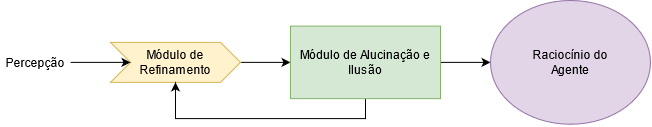
\includegraphics[width=1\textwidth]{images/modelo_geral.png}
    \legend{Fonte: Autor.}
    \label{fig:method}
\end{figure}

\section{Módulo de Refinamento}

\label{refinamento}

O módulo de refinamento funciona como uma primeiro filtro para que percepções indesejadas pelo agente não cheguem até seu ciclo de raciocínio. O processo de refinamento é descrito pela Definição \ref{def:refinamento}.

O processo de refinamento não é obrigatório. Caso não seja de interesse de uma determina implementação do HAIL refinar suas percepções, basta que a função do módulo de refinamento seja a função identidade $f(x) = x$, possuindo assim $\rho = p$.

\begin{example}
    Continuando o exemplo \ref{example::robo2}, as estrelas não fazem parte da área de atuação desse robô, e portanto para otimizarmos o processo de empacotamento é possível utilizar o módulo de refinamento para reduzir a informação desnecessárias enviadas para o raciocínio do agente. Nesse exemplo, o HAIL pode ser implementado com uma função $\theta$ que realiza uma filtragem simbólica, removendo as percepções que não fazem parte do contexto. O conjunto de percepções $p$ passa pelo processo de filtragem e retorna $\rho$. Neste exemplo, sendo $s$ o conjunto de percepções possíveis envolvendo estrelas, a função de refinamento possui um comportamento tal que o conjunto $p$ sob a operação $\theta$ retorna $\rho = p \cap \overline{s}$, ou seja, o agente possui um filtro que remove as percepções que envolvem estrelas.
    
    Por exemplo, vamos supor que o agente recebe o conjunto $p_i$ de percepções, composto por $\{circulo(listrado), triangulo(liso), estrela(amarela)\}$. A operação $\theta$ vai remover de $p_i$ os elementos contidos no conjunto $s$ de possíveis percepções envolvendo estrelas, conforme foi descrito anteriormente. Portanto, a saída do bloco de percepções será $\rho = \{circulo(listrado), triangulo(liso)\}$.
    
\end{example}{}

\section{Módulo de alucinação e ilusão}

\begin{figure}[h]
    \centering
    \caption{Módulo de alucinação e ilusão.}
    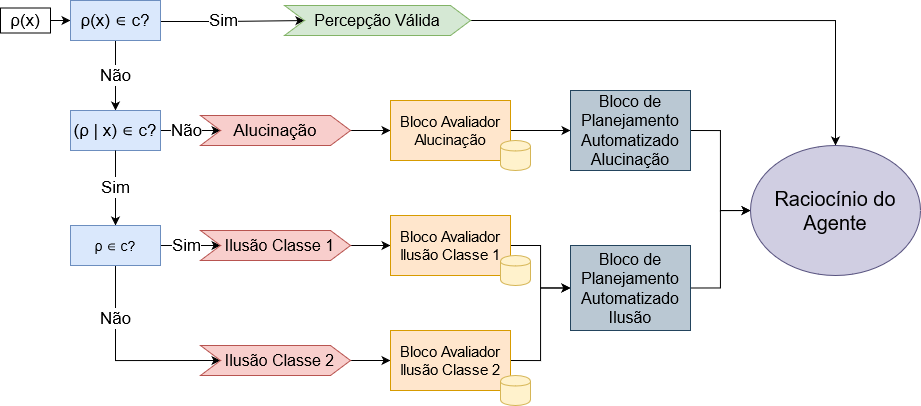
\includegraphics[width=1\textwidth]{images/diagrama-modelo.png}
    \legend{Fonte: Autor.}
    \label{fig:model}
\end{figure}
 
 A Figura \ref{fig:model} apresenta um diagrama do funcionamento do módulo de alucinação e ilusão. Sua função é receber todas as percepções que passaram pelo processo de refinamento, e detectar quais delas são anomalias. Para isso, primeiro cada percepção $\rho(x)$ da entrada $\rho$ (o conjunto de percepções filtradas) é dirigida para o decisor 1. O primeiro decisor responde a pergunta: ``A percepção recebida faz parte do contexto do agente?''. Caso a resposta for sim, consideramos a percepção como válida, e ela é enviada para o raciocínio do agente. Caso a resposta seja não, consideramos $\rho(x)$ uma anomalia, e enviamos ela para o segundo decisor, que responde a pergunta: ``O corpo ou o argumento do predicado $\rho(x)$ faz parte do contexto do agente?''. Caso a resposta seja não, concluímos que a anomalia é uma alucinação. Caso contrário, ela é considerada uma ilusão e é enviada para o terceiro decisor. O terceiro decisor responde a pergunta: ``O corpo do predicado $\rho(x)$ faz parte do contexto do agente?''. Caso a resposta for sim, a ilusão é considerada uma ilusão classe 1, caso contrário, é considerado uma ilusão classe 2. Essa cadeia de decisores pode ser representada pelo Algoritmo \ref{algorithm:decisor}.

\begin{algorithm}[H]
\Entrada{contexto \textit{c} do agente, percepção $\rho(x)$}
\Inicio{
 \label{algorithm:decisor}
  \uSe{$\rho(x)$ está em \textit{c}}{
  $\rho(x)$ é uma percepção válida\;
  }\uSenaoSe{nem $\rho$ nem $x$ estão em c}{
  $\rho(x)$ é uma alucinação\;
  }\uSenaoSe{$\rho$ está em \texttt{c}}{
  $\rho(x)$ é uma ilusão classe 1\;
  }\Senao{$\rho(x)$ é uma ilusão classe 2}
}
 \caption{Funcionamento dos decisores do módulo de alucinação e ilusão.}
\end{algorithm}

% \begin{algorithm}[H]
% \SetKwInOut{Input}{input}
% \Input{agent context \textit{c}, perception $\rho(x)$}

%   \uIf{$\rho(x)$ is in \textit{c}}{
%   $\rho(x)$ is a valid perception\;
%   }\uElseIf{neither $\rho$ nor $x$ is in c}{
%   $\rho(x)$ is a hallucination\;
%   }\uElseIf{$\rho$ is in \texttt{c}}{
%   $\rho(x)$ is an illusion class 1\;
%   }\Else{$\rho(x)$ is an illusion class 2}
%  \label{algorithm:decisor}
%  \caption{Funcionamento dos decisores do módulo de alucinação e ilusão.}
% \end{algorithm}

\begin{example}
    Para entender como as percepções são tratadas pelos decisores, vamos supor algumas entradas possíveis para o agente de nossos exemplos. Vamos analisar dois casos, uma percepção válida e uma anomalia:
    
    \begin{itemize}
        \item \texttt{quadrado(riscado)} -- Essa é uma percepção completamente válida dentro do contexto do agente, pois ele possui um plano específico para tratá-la, que é empacotar o objeto com o papel vermelho, portanto vai fazer parte do conjunto de percepções refinadas $\rho$. Após sair do módulo de refinamento percepções, a percepção é recebida como entrada pelo decisor 1, que detecta que existe um plano específico para tratar da entrada, portanto a percepção é considerada válida e é diretamente enviada para o raciocínio do agente.
        
        \item \texttt{lua(serrilhada)} --  Lua não é um item que deveria ser percebido pelo agente, pois não faz parte dos itens que deveriam ser inseridos na esteira. Todavia, a função de refinamento de nosso agente simplesmente remove as percepções que envolvem estrelas, fazendo com que a percepção \texttt{lua(serrilhada)} chegue ao módulo de alucinação e ilusão. Dentro desse módulo, quando ela chega ao decisor 1, é classificada como anomalia, pois não faz parte do contexto do agente. Em seguida, a percepção é enviada para o decisor 2, que verifica que nem \texttt{lua} nem \texttt{serrilhada} fazem parte do contexto do agente, ou seja, é uma alucinação. Uma vez detectada a alucinação, a percepção segue para o bloco avaliador.
    \end{itemize}
    \label{example:modulo}

\end{example}{}

\subsection{Bloco avaliador}

Após uma anomalia ser classificada, ela é enviada para um bloco avaliador, que tratará de decidir qual anomalia pode ser considerada relevante para ser usada no planejamento automatizado e quais podem ser descartadas. De acordo com a implementação do módulo de refinamento, as percepções que são classificadas como anomalias podem ser utilizadas para otimizar o processo de refinamento.

Em nosso modelo, utilizamos três blocos avaliadores: um para alucinações, um para ilusões classe 1 e outro para ilusões classe 2. Eles são separados para permitir que a prioridade de tratamento de alucinações seja definida individualmente, de acordo com a necessidade do agente que implementa o modelo.

O objetivo do bloco avaliador é decidir quando alucinações e ilusões que foram recebidas devem ser processadas, evitando que o planejamento automatizado que será realizado em seguida tenha impacto no tempo de execução de um ciclo de raciocínio do agente. Para isso, utilizamos uma lista ordenada por peso como escalonador. O principio do funcionamento da lista ordenada por peso é o mesmo de uma fila, \textit{first in first out} (FIFO), mas atribui um peso a cada entrada que aumenta quando novos elementos iguais são inseridos. Quando um elemento é inserido pela primeira vez na fila, ele recebe o peso 1, e quando uma cópia do mesmo elemento é inserida o elemento tem seu peso aumentado em 1, como mostra a Figura \ref{filaPonderada}. Quando uma operação de remoção é executada, o elemento de maior peso é removido. Se dois ou mais elementos tiverem o maior peso, aquele que foi inserido primeiro é removido.

O bloco avaliador seleciona quando uma percepção deve ser tratada através de uma função matemática, levando em conta o tempo médio de processamento de uma percepção válida e de uma anomalia. Além desse funcionamento básico, o bloco avaliador ainda contém um mecanismo para remover anomalias classificadas com irrelevantes para o sistema, através de uma função de limpeza. Caso essa função retorne verdadeiro, todos os elementos de peso 1 da sua respectiva lista são removidos. Essas duas funções são descritas com mais detalhes na Seção \ref{section:formalizacao}.

\begin{figure}[h!]
    \centering
    \caption{Exemplo do funcionamento de uma lista ordenada por peso.}
    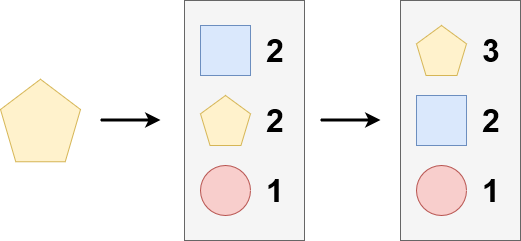
\includegraphics[width=0.8\textwidth]{images/filaPonderada.png}
    \legend{Fonte: Autor}
    \label{filaPonderada}
\end{figure}

\subsection{Bloco de planejamento automatizado}

O bloco de planejamento automatizado é potencialmente a parte mais custosa computacionalmente, o que pode ser um gargalo do sistema, principalmente caso o agente funcione em tempo real e receba um volume muito elevado de percepções por segundo. Um planejamento automatizado implementado de maneira puramente simbólica tende a ser complexo computacionalmente, uma vez que pode considerar milhares de alternativas para o estado de mundo atual, tentando chegar mais perto de seu objetivo. Um processo de planejamento automatizado conexionista é uma alternativa, uma vez que estamos tratando de uma análise incompleta do mundo. Caso seja possível, teorias com maior custo computacional (como criatividade computacional \cite{colton2012computational}) podem ser aplicadas aqui para um resultado ainda mais preciso.

Uma percepção chega ao bloco de planejamento automatizado uma vez que ela seja a primeira na fila ponderada e a função de processamento retorne verdadeiro em sua verificação. De um ciclo para outro, as percepções permanecem na fila, a não ser que sejam descartadas pelo mecanismo de limpeza. Nosso modelo não explicita qual é a ordem que os blocos avaliadores devem processar suas filas para mandar anomalias para o planejamento automatizado (isto é, se deve primeiro ser priorizada as anomalias do bloco avaliador de alucinações, ilusões classe 1 ou ilusões classe 2), ficando a cargo da implementação em questão tomar essa decisão.

\begin{example}
    Para mostrar o caminho que faz uma ilusão, vamos considerar que o agente recebe em duas esteiras a percepção \texttt{triangulo(listrado)}. Não existem triângulos listrados na loja, mas como $\theta$ não filtra essa percepção, ela vai chegar ao decisor 1. 
    
    Os planos do agente são: \texttt{papel(vermelho) :- quadrado(\_) OR circulo(liso)} e 
     \texttt{papel(azul) :- circulo(listrado) OR triangulo(liso)}, e como não existe um plano específico para tratar a percepção \texttt{triangulo(listrado)}, ela é considerada uma anomalia, e é encaminhada ao decisor 2. Como existe um plano para tratar de triângulos lisos, a percepção é então classificada como uma ilusão, e vai para o terceiro decisor. Nele, como o plano trata triângulos, a percepção é considerada uma ilusão classe 1. 
     
     Após a percepção ter sido classificada corretamente, ela é enviada para o bloco avaliador, e é inserida na fila ponderada com peso 1. Depois disso, a percepção da segunda esteira, que é igual a que já foi tratada, chega ao bloco de alucinação e ilusão. Essa percepção vai fazer o mesmo caminho até o bloco avaliador e o peso da anomalia já presente na fila é aumentada para 2. Como duas percepções foram consideradas anomalias, vamos considerar que a função de processamento seja satisfeita, e o bloco avaliador passe essa anomalia para o bloco de planejamento automatizado.
    
    Após uma percepção ser considerada relevante para ser enviada ao planejamento automatizado, ela deve gerar um novo plano para aquela percepção a ser adicionada ao conjunto de planos do agente, e essa percepção então deixará de ser uma anomalia. Ilusões e alucinações tem blocos de planejamento automatizado separados para permitir que duas implementações completamente diferentes sejam utilizadas de acordo com a função do agente e suas particularidades. 
    
    Retomando o exemplo \ref{example:modulo}, no segundo caso, quando o planejamento automatizado de alucinações recebe a percepção \texttt{lua(serrilhada)}, um processo de planejamento automatizado deve ser executado. Para esse exemplo, consideremos um planejamento automatizado puramente simbólico, que analisa uma grande quantidade de estados futuros possíveis para o ambiente em que o robô está inserido e seleciona aquele que será mais eficiente para que o agente se aproxime de seu objetivo principal (terminar de empacotar os itens). Isso é extremamente custoso, mas como alucinações são muito raras para esse agente em questão, pois ele já elimina as percepções inválidas reconhecidas no projeto durante o refinamento, não terá um impacto grande no desempenho do agente. No exemplo, é possível que a lua seja um objeto novo que está sendo vendido, portanto, o agente precisa embalar esse item. Ao detectar uma semelhança entre a lua serrilhada e o circulo listrado, o planejamento automatizado pode determinar que esse novo objeto deve ser embalado com o papel azul, criando assim um novo plano da forma \texttt{papel(azul) :- lua(serrilhada)} é adicionado, e \texttt{lua(serrilhada)} deixa de ser uma alucinação.

    No caso da percepção \texttt{triângulo(listrado)}, o agente poderia ter um bloco de planejamento automatizado baseado em uma rede bayesiana, uma vez que ilusões podem ser muito mais comuns e o agente já tem uma breve noção do que deve ser feita com objetos do tipo. \texttt{triângulo(listrado)} pode ser um novo item a venda na loja, e como já foi verificado em duas esteiras diferentes, faz sentido que ele não seja uma mera falha de sensores. Assim, o planejamento automatizado pode inferir o plano \texttt{triângulo(listrado) -> empacotar}, permitindo que o agente tenha um aprendizado dinâmico resultado da adição de um novo plano em seu conjunto de planos. Assim como no caso da ilusão, uma vez que esse plano novo foi adicionado a percepção original deixa de ser uma anomalia, uma vez que faz parte do contexto em que o agente está trabalhando.
    \label{example::planejamento}
\end{example}{}

\section{Raciocínio do agente}

O raciocínio do agente se refere a todos os fatores externos do modelo de revisão de percepções pertencentes ao agente, principalmente a arquitetura cognitiva utilizada para implementá-lo. Em um agente qualquer, o raciocínio é alimentado principalmente pelas percepções. Outras fontes de conhecimento, como comunicação, podem existir também, mas para o modelo HAIL consideramos toda forma de entrada como percepção. Em um agente que implemente o modelo HAIL, o raciocínio recebe tanto as percepções consideradas válidas pelo módulo de alucinação e ilusão quanto os novos planos criados a partir do planejamento automatizado.